\newpage
\section{Experiment Thermal Analysis} \label{sec:appI}
\subsection{Component Temperature Ranges}

Table {\ref{tab:thermal-table}}, below covers the thermal ranges of all components included in the experiment's flight stage as listed in Section \ref{sec:experiment-components}:



%Added this space to help us see all of the numbers. This "Track changes" sign blocks them every time!


\begin{longtable}{|m{1cm}|m{3.5cm}|m{1.3cm}|m{1.3cm}|m{1.4cm}|m{1.3cm}|m{1.3cm}|m{1.3cm}|}
\hline
\multirow{2}{*}{\textbf{ID}} & \multirow{2}{*}{\textbf{Components}}                                 & \multicolumn{2}{l|}{\textbf{Operating ($\degree{C}$)}} & \multicolumn{2}{l|}{\textbf{Survivable ($\degree{C}$)}} & \multicolumn{2}{l|}{\textbf{Expected ($\degree{C}$)}} \\ \cline{3-8} &   & Min.  & Max.  & Min.  & Max.  &  Min.   &  Max.            \\ \hline
E1 & Arduino Due & -40 & 85 & -60 & 150 & -15.7 & 54.0 \\ \hline
E2 & Ethernet Shield & -40 & 85 & -65 & 150 & -15.7 & 54.0 \\ \hline
E3 & Miniature diaphragm air pump & 5 & 40 & -10 & 40 & 10 & 34.9 \\ \hline
E4 & Pressure Sensor & -40 & 85 & -40 & 125 & -15.7 & 54.0 \\ \hline
E5 & Sampling Valve (inlet and outlet 1/8"" female) & -20 & 68 & -20\textsuperscript{\ref{fn:erik}} & 68\textsuperscript{\ref{fn:erik}} & -15 & 20 \\ \hline
E6 & Airflow sensor AWM43300V & -20 & 70 & -20\textsuperscript{\ref{fn:erik}} & 70\textsuperscript{\ref{fn:erik}} & -8.8 & 34.9 \\ \hline
E7 & Heater ($12.7\times 50.8 mm$) & -200 & 200 & -200\textsuperscript{\ref{fn:erik}} & 200\textsuperscript{\ref{fn:erik}} & -20 & 36 \\ \hline
%E8 & Voltage Regulator & -40 & 125 & -40\textsuperscript{\ref{fn:erik}} & 125\textsuperscript{\ref{fn:erik}} & -30.62 & 34.93 \\ \hline
E9 & Temperature Sensor & -55 & 125 & -65 & 150 & -19.7 & 43 \\ \hline
E10 & DCDC 24 V & -40 & 85 & -55 & 125 & -15.7 & 54.0 \\ \hline
E12 & Micro SD & -25 & 85 & -200\textsuperscript{\ref{fn:erik}} & 200\textsuperscript{\ref{fn:erik}} & -15.7 & 54.0 \\ \hline
E13 & Logic CAT5E & -55 & 60 & -55\textsuperscript{\ref{fn:erik}} & 60\textsuperscript{\ref{fn:erik}} & -34 & 15 \\ \hline
% E14 & Resistors (33, 150 and 100 ohm) & -55 & 155 & (-55)\textsuperscript{\ref{fn:erik}} & (155)\textsuperscript{\ref{fn:erik}} & TBD\textsuperscript{\ref{fn:ivan}} & TBD\textsuperscript{\ref{fn:ivan}} \\ \hline
% E15 & Capacitors $(0.1 \mu$ F and $10 \mu$ F) & -30 & 85 & -55 & 125 & -55\textsuperscript{\ref{fn:erik}} & 125\textsuperscript{\ref{fn:erik}} & -15.7 & 54.0 \\ \hline
E16 & MOSFET for current control & -55 & 175 & -55 & 175 & -15.7 & 54.0 \\ \hline
E17 & Diodes for DCDC converters & -65 & 175 & -65\textsuperscript{\ref{fn:erik}} & 175\textsuperscript{\ref{fn:erik}} & -15.7 & 54.0 \\ \hline
E18 & 3.3V LED & -40 & 85 & -40\textsuperscript{\ref{fn:erik}} & 85\textsuperscript{\ref{fn:erik}} & -15.7 & 54.0 \\ \hline 
E19 & 15-pin D-SUB Female connector with pins & -55 & 120 & -200\textsuperscript{\ref{fn:erik}} & 200\textsuperscript{\ref{fn:erik}} & -15.7 & 54.0 \\ \hline
E20 & 9-pin D-SUB Female connector with pins & -55 & 120  & -200\textsuperscript{\ref{fn:erik}} & 200\textsuperscript{\ref{fn:erik}} & -15.7 & 54.0 \\ \hline
E21 & 9-pin D-SUB Female connector with soldering cups & -55 & 105 & -55\textsuperscript{\ref{fn:erik}} & 105\textsuperscript{\ref{fn:erik}} & -15.7 & 54.0 \\ \hline
E22 & 9-pin D-SUB Male connector with soldering cups & -55 & 105 & -55\textsuperscript{\ref{fn:erik}} & 105\textsuperscript{\ref{fn:erik}} & -15.7 & 54.0 \\ \hline
E23 & 15-pin D-SUB Male connector with soldering cups & -55  & 105 & -55\textsuperscript{\ref{fn:erik}} & 105\textsuperscript{\ref{fn:erik}} & -15.7 & 54.0 \\ \hline
E24 & 9-pin D-SUB backing & -40 & 120 & -40\textsuperscript{\ref{fn:erik}} & 120 & -15.7 & 54.0  \\ \hline
E25 & 15-pin D-SUB backing & -40 & 120 & -40\textsuperscript{\ref{fn:erik}} & 120 & -15.7 & 54.0  \\ \hline
% E26 & Wall mounting bolts & TBD\textsuperscript{\ref{fn:ivan}} & TBD\textsuperscript{\ref{fn:ivan}} & TBD\textsuperscript{\ref{fn:ivan}} & TBD\textsuperscript{\ref{fn:ivan}} & TBD\textsuperscript{\ref{fn:ivan}} & TBD\textsuperscript{\ref{fn:ivan}} \\ \hline
%E27 & D-SUB cable CAC to AAC & -40 & 85 & -55 & 125 & -40 & 40 \\ \hline
E28 & 3.3 Zener diode & -65 & 175 & -65\textsuperscript{\ref{fn:erik}} & 175\textsuperscript{\ref{fn:erik}} & -15.7 & 54.0 \\ \hline
E29 & Male connector on PCB & -40 & 85 & -40\textsuperscript{\ref{fn:erik}} & 85 & -15.7 & 54.0 \\ \hline
E30 & Female connector from wall & -40 & 85 & -40\textsuperscript{\ref{fn:erik}} & 85 & -50.7 & 15 \\ \hline
E31 & Grounding contact & -55 & 125 & -55\textsuperscript{\ref{fn:erik}} & 125\textsuperscript{\ref{fn:erik}} & -50.7 & 15 \\ \hline
E32 & Logic CAT5 E-link for inside box &-55 & 60 & -55\textsuperscript{\ref{fn:erik}} & 60\textsuperscript{\ref{fn:erik}} & -34 & 15 \\ \hline
E33 & Signal Wires & -60 & 200 & -60\textsuperscript{\ref{fn:erik}} & 200\textsuperscript{\ref{fn:erik}} & -34 & 15 \\ \hline
E34 & Flushing valve (inlet and outlet 1/8"" female) & -20 & 68 & -20\textsuperscript{\ref{fn:erik}} & 68 & -7.4 & 25.8 \\ \hline
E35 & Valves manifold (outlet 1/8"" female) & -10 & 50 & -10\textsuperscript{\ref{fn:erik}} & 50\textsuperscript{\ref{fn:erik}} & 3 & 18 \\ \hline
E36 & Power wire black & -60 & 200 & -60\textsuperscript{\ref{fn:erik}} & 200\textsuperscript{\ref{fn:erik}} & -34 & 15 \\ \hline
% E44 & Heat shrinking tube 2.5 x 1mm & -55 & 125 & (-55)\textsuperscript{\ref{fn:erik}} & (125)\textsuperscript{\ref{fn:erik}} & TBD\textsuperscript{\ref{fn:ivan}} & TBD\textsuperscript{\ref{fn:ivan}} \\ \hline
%E45 & 25-pin D-SUB female connector with pins & -10 & 90 & -10\textsuperscript{\ref{fn:erik}} & 90\textsuperscript{\ref{fn:erik}} & -8.77 & 24.01 \\ \hline
%E46 & 25-pin D-SUB male connector with soldering cups & -10 & 90 & -10\textsuperscript{\ref{fn:erik}} & 90\textsuperscript{\ref{fn:erik}} & -8.77 & 24.01 \\ \hline
%E47 & 25-pin D-SUB backing & -10 & 90 & -10\textsuperscript{\ref{fn:erik}} & 90\textsuperscript{\ref{fn:erik}} & -8.77 & 24.01 \\ \hline
E48 & Power wire red & -60 & 200 & -60\textsuperscript{\ref{fn:erik}} & 200
\textsuperscript{\ref{fn:erik}} & -34 & 15  \\ \hline
% E49 & Potentiometer 1k ohm & -55 & 125 & (-55)\textsuperscript{\ref{fn:erik}} & (120)\textsuperscript{\ref{fn:erik}} & TBD\textsuperscript{\ref{fn:ivan}} & TBD\textsuperscript{\ref{fn:ivan}} \\ \hline
E50 & 6-pin male & -55 & 105 & -55\textsuperscript{\ref{fn:erik}} & 105\textsuperscript{\ref{fn:erik}} & -8.8 & 24.0  \\ \hline
E51 & 8-pin male single row header& -40 & 105 & -40\textsuperscript{\ref{fn:erik}} & 105\textsuperscript{\ref{fn:erik}} & -8.8 & 24.0  \\ \hline
E52 & 10-pin male single row header & -55 & 105 & -55\textsuperscript{\ref{fn:erik}} & 105\textsuperscript{\ref{fn:erik}} & -8.8 & 24.0  \\ \hline
E53 & 36-pin male double row header & -40 & 105 & -40 & 125 & -8.8 & 24.0  \\ \hline
E54 & 12 V DC/DC converter & -40 & 85 & -55 & 125 & -15.7 & 54.0  \\ \hline
E55 & 50 k$\Omega$ Potentiometer & -55 & 125 & -55\textsuperscript{\ref{fn:erik}} & 125\textsuperscript{\ref{fn:erik}} & -15.7 & 54.0  \\ \hline
E56 & Static pressure sensor & -40 & 120 & -40\textsuperscript{\ref{fn:erik}} & 120\textsuperscript{\ref{fn:erik}} &  -8.8 & 34.9 \\ \hline
E57 & Connector for static pressure sensor & -25 & 80 & -25\textsuperscript{\ref{fn:erik}} & 80\textsuperscript{\ref{fn:erik}} &  -8.8 & 34.9 \\ \hline
E58 & PCB & -50 & 110 & -50\textsuperscript{\ref{fn:erik}} & 110\textsuperscript{\ref{fn:erik}} & -15.7 & 54.0 \\ \hline
E59 & Pressure Sensor PCB & -50 & 110 & -50\textsuperscript{\ref{fn:erik}} & 110\textsuperscript{\ref{fn:erik}} & -50 & 39 \\ \hline


\caption{Table of Component Temperature Ranges.}
\label{tab:thermal-table}
\end{longtable}
\raggedbottom










\raggedbottom

\subsection{Thermal equations}

\subsubsection{Variables and Tables}
\begin{table}[H]
    \centering
    \begin{tabular}{|c|c|c|c|}
        \hline
        \textbf{Variable} & \textbf{Description} & \textbf{Unit} & \textbf{Value} \\ \hline
        $\alpha_{Al}$ & Absorption of aluminum & - & 0.3 \\ \hline
        S & Solar constant & $\frac{W}{m^2}$ & 1362 \\ \hline
        $A_{Sun}$ & Area affected by the sun & $m^2$ & 0.28 \\ \hline
        Albedo & Albedo coefficient & - & 0.15 \\ \hline
        $A_{Albedo}$ & Area affected by the albedo & $m^2$ & 0.65 \\ \hline
        $\varepsilon_{Earth}$ & Emissivity of Earth & - & 0.95 \\ \hline
        $A_{IR}$ & Area affected by the IR flux & $m^2$ & 0.65 \\ \hline
        $IR_{25km}$ & Earth IR flux at 25 km & $\frac{W}{m^2}$ & 220 \\ \hline
        P & Dissipated power from electronics & W & varies \\ \hline
        h & Convection heat transfer constant & $\frac{W}{m^2 \cdot K}$ & 18 \\ \hline
        K & Scaling factor for convection & - & varies \\ \hline
        $A_{Convection}$ & Area affected by the convection & $m^2$ & 1.3 \\ \hline
        $\sigma$ & Stefan-Boltzmann constant & $\frac{W}{m^2 \cdot K^4}$ & $5.67051 \cdot 10^{-8}$ \\ \hline
        $A_{Radiation}$ & Radiating area & $m^2$ & 1.3\\ \hline
        $\varepsilon_{Al}$ & Emissivity of aluminum & - & 0.09 \\ \hline
        $T_{Out}$ & Temperature wall outside & $K$ & varies \\ \hline
        $T_{Inside}$ & average uniform temperature inside & $K$ & varies \\ \hline
        $T_{Ambient}$ & Ambient temperature outside & $K$ & varies \\ \hline
        $T_{Ground}$ & Temperature of the ground & $K$ & 273 \\ \hline
        $k_{Al}$ & Thermal conductivity of aluminum & $\frac{W}{m\cdot K}$ & 205 \\ \hline
        $k_{PS}$ & Thermal conductivity of polystyrene foam & $\frac{W}{m\cdot K}$ & 0.03 \\ \hline
        $L_{Al}$ & Thickness of aluminum sheeting & $m$ & 0.0005 \\ \hline
        $L_{PS}$ & Thickness of polystyrene foam & $m$ & varies \\ \hline
        $P_{Ground}$ & Pressure at ground & $Pa$ & $101.33 \cdot 10^3$ \\ \hline
        $P_{25km}$ & Pressure at $25 km$ & $Pa$ & $2.8 \cdot 10^3$ \\ \hline
    \end{tabular}
    \caption{Variables Used in Thermal Calculation.}
    \label{tab:thermal-variables}
\end{table}

\begin{table}[H]
\centering

\begin{tabular}{ll}
\hline
\multicolumn{1}{|l|}{\textbf{Wall part}}              & \multicolumn{1}{l|}{\textbf{Thickness (m)}} \\ \hline
\multicolumn{1}{|l|}{Aluminum sheet}         & \multicolumn{1}{l|}{0.0005}        \\ \hline
                                             &                                    \\ \cline{1-1}
\multicolumn{1}{|l|}{AAC (Styrofoam)}        &                                    \\ \hline
\multicolumn{1}{|l|}{Vertical}               & \multicolumn{1}{l|}{0.02}          \\ \hline
\multicolumn{1}{|l|}{Horizontal}             & \multicolumn{1}{l|}{0.02}          \\ \hline
\multicolumn{1}{|l|}{Top/Bottom}             & \multicolumn{1}{l|}{0.03}          \\ \hline
                                             &                                    \\ \cline{1-1}
\multicolumn{1}{|l|}{CAC (Styrofoam)}        &                                    \\ \hline
\multicolumn{1}{|l|}{Horizontal towards AAC} & \multicolumn{1}{l|}{0.02}          \\ \hline
\multicolumn{1}{|l|}{All other walls}        & \multicolumn{1}{l|}{0.05}          \\ \hline
\end{tabular}
\caption{The Different Wall Thicknesses Used for AAC and CAC.}
\label{tab:Wall-thickness-AAC-CAC}
\end{table}

%\begin{table}[H]
%\centering
%\caption{Dissipated power at the different stages.}
%\label{tab:dissipated-power-thermal}
%\begin{tabular}{|l|l|l|}
%\hline
%\multirow{2}{*}{Critical stage} & \multicolumn{2}{l|}{Dissipated power (W)} \\ \cline{2-3} 
%                                & Worst case       & Average case       \\ \hline
%Launch pad                      & 7.589            & 5.083              \\ \hline
%Early ascent                    & 11.499           & 8.993              \\ \hline
%Sampling ascent                 & 13.499           & 13.397             \\ \hline
%Float                           & 11.499           & 8.993              \\ \hline
%Sampling descent                & 13.499           & 13.397             \\ \hline
%Shutdown descent                & 2.167            & 2167               \\ \hline
%Landed                          & 0                & 0                  \\ \hline
%\end{tabular}
%\end{table}
%The difference in dissipated power is depending if heaters need to be on or not.


\subsection{Thermal calculations in MATLAB}
For the MATLAB calculations, a few assumptions were made. They were as follows:
\begin{itemize}
    \item Taking the average of MATLAB calculations for calculations with or without sunlight.
    \item Calculating the average temperature on the outside wall of the experiment.
    \item Assuming the inner temperature at the bags section is uniform.
    \item Ignoring the pipes letting cold air into the experiment.
    \item Assuming no interference between the two experiment boxes.
    \item All conduction was uniform from the inside.
    \item Assume steady flow through the walls from conduction.
    \item Assume radiation and convection from/on 6 walls not 5.
\end{itemize}

\subsubsection{Solar flux and Albedo}
The albedo is the reflected solar flux from earth so it was put into the same equation as the solar flux. It was assumed that the sun hit two sides of the experiment at a $45\degree$ angle at all times while over 10 km altitude. In the middle of October at the time of launch the sun was expected to hit the experiment with a maximum inclination of $15\degree$ from the horizon.
\begin{equation*}
    Q_{Sun+Albedo} = \alpha_{Al}\cdot S \cdot cos(15) \cdot (A_{Sun} \cdot cos(45) + Albedo \cdot A_{Albedo})
\end{equation*}

\subsubsection{Conduction}
For calculating the outer walls temperature, the assumption of steady flow through walls was used.
\begin{equation*}
    Q_{Conduction} = [\text{Steady flow through wall}] = \text{Dissipated power} = P
\end{equation*}

\subsubsection{Earth IR flux}
The earth IR flux is the flux that comes from earth as a black body radiating. It was calculated from the determined IR flux at ground level then scaled to the altitude the experiment would reach. The following equations were found from \cite{BalloonAscent}:
\begin{gather*}
    IR_{Ground} = \varepsilon_{earth} \cdot \sigma \cdot T_{ground}^4 \\
    \tau_{atmIR} = 1.716 - 0.5\cdot \Bigg[e^{-0.65\frac{P_{25km}}{P_{ground}}} + e^{-0.95\frac{P_{25km}}{P_{ground}}}\Bigg] \\
    IR_{25km} = \tau_{atmIR} \cdot IR_{Ground}
\end{gather*}
After the IR was calculated for the floating altitude it was put into the following equation. 
\begin{equation*}
    Q_{IR} = \varepsilon_{earth} \cdot A_{IR} \cdot IR_{25km}
\end{equation*}

\subsubsection{Radiation}
It was assumed that the experiment would experience radiation from all 6 sides. In reality it would experience radiation from 5 sides because the CAC box will be in contact with one of the AAC box's sides. It was decided to leave the simulation with input from the 6 sides for the calculations in order to compensate for having no holes to let cold air in to the pump.
\begin{equation*}
    Q_{Radiation} = \sigma \cdot \varepsilon_{Al} \cdot A_{Radiation} \cdot (T_{Out}^4 - T_{Ambient}^4 )
\end{equation*}

\subsubsection{Convection}
At an altitude of 25 km there is far lower air density than at sea level. This therefore gave a scaling factor $K$ that had to be taken into account when calculating the convection and K can be seen in Table \ref{tab:heat-loss} for different altitudes.
\begin{equation*}
    Q_{Convection} = h \cdot K \cdot A_{Convection} \cdot (T_{Out} - T_{Ambient})
\end{equation*}

The equation for approximating the heat transfer coefficient for air was outlined as:
\begin{equation*}
h = 10.45 - v + 10\cdot\sqrt{v}
\end{equation*}
Where $v$ is the velocity of the fluid medium.

As the balloon was expected to rise at approximately $5 m/s$ for the duration of the Ascent Phase, the starting value for the convective heat transfer coefficient $h$ was expected to be $27.811$, assuming negligible wind currents perpendicular to the direction of ascent. %I will probably move this paragraph to our Thermal Design section, since this is important information.

The equations used to obtain the value of $K$ are listed below:

\begin{equation*}
F(T_{sea}, T_{alt}) = \big(\frac{k_{alt}}{k_{sea}}\big)^{1-n}\times \Big[\Big(\frac{\beta_{alt}}{\beta_{sea}}\Big)\times \Big(\frac{\mu_{sea}}{\mu_{alt}}\Big)\times \Big(\frac{c_{p-alt}}{c_{p-sea}}\Big)\times \Big(\frac{\rho(T_{alt})}{\rho(T_{sea})}\Big)^{2}\Big]^{n}
\end{equation*}

Where:
\begin{itemize}
    \item $n$ is an exponent value dependent on the turbulence of the fluid medium ($\frac{1}{4}$ for laminar flow and $\frac{1}{3}$ for turbulent flow)
    \item $k$ is the thermal conductivity of the air
    \item $\beta$ is the thermal expansion coefficient for air
    \item $\mu$ is the dynamic viscosity of the air
    \item $c_{p}$ is the specific heat capacity of the air at constant pressure
    \item $\rho(T)$ is the density of the air as a function of only temperature difference (i.e. for constant pressure)
    \item "sea" denotes the current variable is represented by its value found at sea level
    \item "alt" denotes the current variable is represented by its value found at a specified altitude
\end{itemize}


The values for $F$ from this equation were then applied to its respective position in the following equation to determine the ratio between the convective heat transfer coefficient $h$ at sea level (assumed to have negligible differences for Esrange ground level) and the same coefficient at a specified altitude:

\begin{equation*}
K = \Big(\frac{\rho(P_{alt})}{\rho(P_{sea})}\Big)^{2n}\times \Big(\frac{\Delta T_{air}}{\Delta T_{sea}}\Big)^{n}\times F(T_{sea}, T_{alt})
\end{equation*}

Where:
\begin{itemize}
    \item $\rho(T)$ is the density of the air as a function of only temperature difference (i.e. for constant pressure)
    \item $\delta T$ is the difference between the temperature of the ambient air and the surface in question
\end{itemize} \\


%Table for convective and radiative heat loss will go here.

Table \ref{tab:heat-loss} combines the previously listed convection and radiation formulae integrated into the MATLAB scripts to determine the convective and radiative heat loss in the worst case for (highest) power dissipation during each stage of the experiment. Additional information on the thermodynamics of the atmosphere was obtained from \textit{Engineering Toolbox} \cite{EngTool} \\





\begin{longtable}{|m{2.5cm}|m{1.6cm}|m{1cm}|m{1.2cm}|m{1.2cm}|m{1cm}|m{1.5cm}|m{1.5cm}|}
\hline

\textbf{Altitude} & \textbf{Case} & \textbf{$T_{amb}$} & \textbf{$K$} & \textbf{$h_{alt}$} & \textbf{$T_{out}$} & \textbf{$Q_{conv}$} & \textbf{$Q_{rad}$} \\ \hline
\multirow{3}{*}{\begin{tabular}[c]{@{}l@{}}Hangar\\ (Preparations)\end{tabular}} & Cold & 283 & 1 & 10.45 & 20.3 & 139.409 & 6.516 \\
 & Expected & 288 & 1 & 10.45 & 25.2 & 139.081 & 6.844 \\
 & Warm & 293 & 1 & 10.45 & 30.2 & 138.743 & 7.182 \\ \hline
\multirow{3}{*}{\begin{tabular}[c]{@{}l@{}}Ground\\ (Stationary)\end{tabular}} & Cold & 263 & 1 & 18 & -0.8 & 215.705 & 4.690 \\
 & Expected & 273 & 1 & 18 & 9.2 & 215.171 & 5.222 \\
 & Warm & 283 & 1 & 18 & 19.2 & 214.600 & 5.790 \\ \hline
\multirow{3}{*}{\begin{tabular}[c]{@{}l@{}}Ground\\ (Launched)\end{tabular}} & Cold & 263 & 1 & 28.945 & -4.2 & 217.528 & 2.884 \\
 & Expected & 273 & 1 & 28.945 & 5.8 & 217.195 & 3.217 \\
 & Warm & 283 & 1 & 28.945 & 15.8 &  216.837 & 3.573 \\ \hline
\multirow{3}{*}{5 km} & Cold & 228 & 0.7868 & 22.774 & -37.6 & 217.979 & 2.430 \\
 & Expected & 263 & 0.8468 & 24.511 & -3.2 &  216.990 & 3.417 \\
 & Warm & 273 & 0.8507 & 24.624 & 6.3 & 216.615 & 3.792 \\ \hline
\multirow{3}{*}{10 km} & Cold & 193 & 0.4882 & 14.131 & -68.1 & 217.916 & 2.480 \\
 & Expected & 223 & 0.5286 & 15.300 & -39.1 & 216.940 & 3.453 \\
 & Warm & 238 & 0.5421 & 15.691 & -24.4 & 216.336 & 4.055 \\ \hline
\multirow{3}{*}{15 km} & Cold & 193 & 0.3300 & 9.552 & -61.9 & 224.325 & 3.961 \\
 & Expected & 233 & 0.3680 & 10.652 & -23.9 & 222.309 & 5.972 \\
 & Warm & 253 & 0.3825 & 11.071 & -4.6 & 221.050 & 7.226 \\ \hline
\multirow{3}{*}{20 km} & Cold & 213 & 0.2401 & 6.950 & -35.6 & 220.777 & 7.430 \\
 & Expected & 243 & 0.2563 & 7.419 & -7.4 & 218.297 & 9.899 \\
 & Warm & 268 & 0.2687 & 7.778 & 16.4 & 215.906 & 12.282 \\ \hline
\multirow{3}{*}{25 km} & Cold & 223 & 0.1683 & 4.871 & -16.0 & 215.482 & 12.549 \\
 & Expected & 253 & 0.1792 & 5.187 & 11.4 & 211.791 & 16.226 \\
 & Warm & 273 & 0.1847 & 5.346 & 30.1 & 208.893 & 19.112 \\ \hline
\multirow{3}{*}{\begin{tabular}[c]{@{}l@{}}Float\\ Phase\end{tabular}} & Cold & 223 & 0.1683 & 3.029 & -1.7 & 190.087 & 19.521 \\
 & Expected & 253 & 0.1792 & 3.226 & 24.1 & 185.077 & 24.530 \\
 & Warm & 273 & 0.1847 & 3.325 & 41.9 & 181.196 & 28.402 \\ \hline
 \multirow{3}{*}{25 km} & Cold & 223 & 0.1683 & 5.173 & -20.3 & 199.514 & 10.633 \\
 & Expected & 253 & 0.1792 & 5.508 & 7.4 & 196.295 & 13.838 \\
 & Warm & 273 & 0.1847 & 5.677 & 26.3 & 193.765 & 16.356 \\ \hline
 \multirow{3}{*}{20 km} & Cold & 213 & 0.2401 & 7.379 & -36.9 & 221.276 & 6.948 \\
 & Expected & 243 & 0.2563 & 7.877 & -8.6 & 218.934 & 9.280 \\
 & Warm & 268 & 0.2687 & 8.258 & 15.2 & 216.672 & 11.534 \\ \hline
 \multirow{3}{*}{15 km} & Cold & 193 & 0.3300 & 10.142 & -63.6 & 216.808 & 3.561 \\
 & Expected & 233 & 0.3680 & 11.310 & -25.4 & 214.974 & 5.389 \\
 & Warm & 253 & 0.3825 & 11.756 & -6.0 & 213.829 & 6.530 \\ \hline
 \multirow{3}{*}{10 km} & Cold & 193 & 0.4882 & 15.004 & -68.8 & 218.074 & 2.326 \\
 & Expected & 223 & 0.5286 & 16.246 & -39.7 & 217.155 & 3.242 \\
 & Warm & 238 & 0.5421 & 16.661 & -25.0 & 216.586 & 3.809 \\ \hline
 \multirow{3}{*}{5 km} & Cold & 228 & 0.7868 & 24.182 & -38.1 & 218.127 & 2.284 \\
 & Expected & 263 & 0.8468 & 26.026 & -3.6 & 217.195 & 3.214 \\
 & Warm & 273 & 0.8507 & 26.145 & 6.4 & 216.841 & 3.567 \\ \hline
 \multirow{3}{*}{\begin{tabular}[c]{@{}l@{}}Ground\\ (Landed)\end{tabular}} & Cold & 263 & 1 & 30.734 & -4.6 & 217.700 & 2.713 \\
 & Expected & 273 & 1 & 30.734 & 5.4 & 217.386 & 3.027 \\
 & Warm & 283 & 1 & 30.734 & 15.4 & 217.049 & 3.363 \\ \hline
 \multirow{3}{*}{\begin{tabular}[c]{@{}l@{}}Ground\\ (Stationary)\end{tabular}} & Cold & 263 & 1 & 18 & -4.8 & 207.753 & 2.586 \\
 & Expected & 273 & 1 & 18 & 5.2 & 207.453 & 2.885 \\
 & Warm & 283 & 1 & 18 & 15.2 & 207.132 & 3.205 \\ \hline
\caption{Table of Predicted Heat Loss.}
\label{tab:heat-loss}
\end{longtable}

\raggedbottom


\subsubsection{Thermal equations}
If there is no incident sunlight on the experiment.
\begin{gather*}
    Q_{IR} + Q_{Conduction} = Q_{Radiation} + Q_{Convection} \\
    \updownarrow \\
    \varepsilon_{earth} \cdot A_{IR} \cdot IR_{25km} + P \\ = \sigma \cdot \varepsilon_{Al} \cdot A_{Radiation} \cdot (T_{Out}^4 - T_{Ambient}^4 ) + h \cdot K \cdot A_{Convection} \cdot (T_{Out} - T_{Ambient})
\end{gather*}
If there is incident sunlight on the experiment, existing parameters stay included, and the parameter $Q_{Sun+Albedo}$ is also included.
\begin{gather*}
    Q_{IR} + Q_{Conduction} + Q_{Sun+Albedo} = Q_{Radiation} + Q_{Convection} \\
    \updownarrow \\
    \varepsilon_{earth} \cdot A_{IR} \cdot IR_{25km} + P + \alpha_{Al}\cdot S \cdot cos(15) \cdot (A_{Sun} \cdot cos(45) + Albedo \cdot A_{Albedo}) \\ = \sigma \cdot \varepsilon_{Al} \cdot A_{Radiation} \cdot (T_{Out}^4 - T_{Ambient}^4 ) + h \cdot K \cdot A_{Convection} \cdot (T_{Out} - T_{Ambient})
\end{gather*}
From these equations $T_{Out}$ could be calculated and it was found to be the average temperature on the aluminum sheets facing the outside air.
After $T_{Out}$ was found, the inner temperature could be calculated by determining the heat transfer through the wall.
\begin{gather*}
    P = \frac{T_{Inside} - T_{Outside}}{A \cdot (\frac{L_{Al}}{k_{Al}} + \frac{L_{PS}}{k_{PS}})} \\
     \updownarrow \\
    T_{Inside} = P \cdot A \cdot (\frac{L_{Al}}{k_{Al}} + \frac{L_{PS}}{k_{PS}}) + T_{Outside}
\end{gather*}
$T_{Inside}$ was then assumed to be the uniform air temperature in the experiment.



\subsubsection{Trial run with BEXUS 25 air temperature data for altitudes}
The air temperature data varying over altitude from previous BEXUS flights could be found on the REXUS/BEXUS website. To do a simulated test flight for the calculations done in MATLAB (with the intention of seeing how the temperature profile would appear for a real flight), it was calculated and plotted in with data from BEXUS 25 flight.
Because of it originally having approximately 42000 data points, the profile had to be scaled down. Only every $25^{th}$ data point was used to reduce processing time and this resulted in little detail loss. In Figure \ref{fig:thermal-testflight-AAC}, the TUBULAR test flight is the uniform temperature on the inside with a insulation consisting as specified in Table \ref{tab:Wall-thickness-AAC-CAC}.

\begin{figure}[H]
    \begin{align*}
        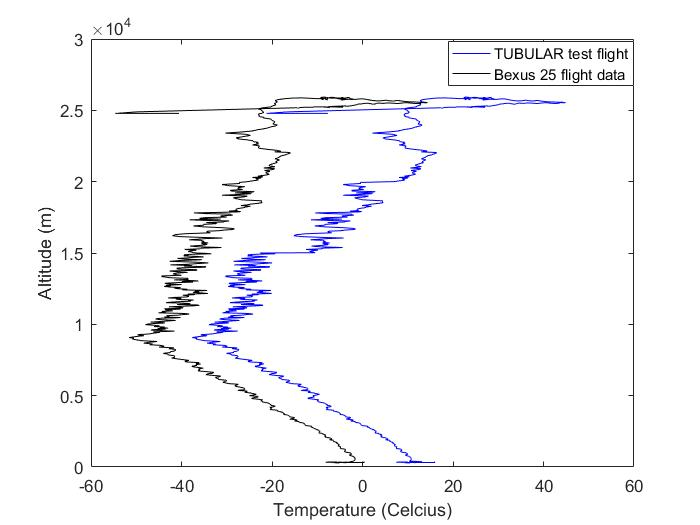
\includegraphics[width=1\linewidth]{appendix/img/Thermal/AAC-test-flight.jpg}
    \end{align*}
    \caption{Simulated Test Flight of TUBULAR AAC Box with Data From BEXUS 25.}
    \label{fig:thermal-testflight-AAC}
\end{figure}
When the data was found it was checked in ANSYS to determine and add heaters to control the most critical parts of the model.

\subsubsection{Trial flight for the CAC} \label{sssec:CAC-trial-flight}
The CAC box did not require as much thermal design as the AAC box. The only part to be considered was the valve, which had a lower limit of the operating temperature of $-10\degree{ C}$. It would not be a problem because the valve would open just prior launch and have current running through it throughout the whole flight --- heating it self up. If the thermal analysis was proven wrong by a test, showing that it was not sufficient to use only self-heating, a heater could be applied at a later date. The passive thermal design for the CAC box would consist of aluminum sheets and Styrofoam as specified in \ref{tab:Wall-thickness-AAC-CAC}.
\begin{figure}[H]
    \begin{align*}
        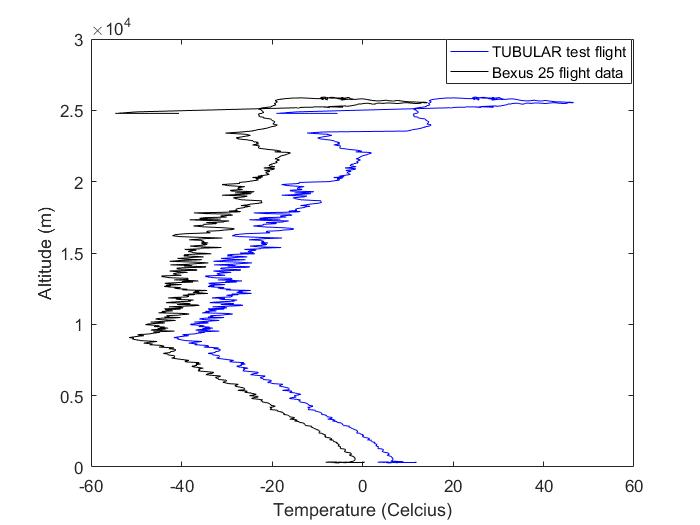
\includegraphics[width=1\linewidth]{appendix/img/Thermal/CAC-test-flight.jpg}
    \end{align*}
    \caption{Simulated Test Flight of TUBULAR CAC Box with Data From BEXUS 25.}
    \label{fig:thermal-testflight-CAC}
\end{figure}

\subsubsection{MATLAB Conclusion}
By running the MATLAB script, the hottest and coldest case for $0.02 m$ on the wall and $0.03 m$ on the top and bottom of the Styrofoam could be found for ascent and descent sampling. The thermal conductivity of Styrofoam is $k=0.03$. In Table \ref{tab:temperature-sampling-ascent-descent} it is shown the hottest and coldest case of temperature on the inside when samples should be taken. The hottest and coldest cases are taken from Figure \ref{fig:thermal-testflight-AAC}.


\begin{table}[H]
\centering
\begin{tabular}{l|l|l|l|l|}
\cline{2-5}
\multirow{2}{*}{}               & \multicolumn{2}{l|}{\textbf{Ascent}} & \multicolumn{2}{l|}{\textbf{Descent}} \\ \cline{2-5} 
                                & Coldest      & Hottest      & Coldest       & Hottest      \\ \hline
\multicolumn{1}{|l|}{AAC}       & -11.39       & 16.41        & -30.28        & -4.393       \\ \hline
\multicolumn{1}{|l|}{Outer air} & -38.22       & -15.9        & -44.41        & -38.18       \\ \hline
\end{tabular}
\caption{The Sampling Temperature Ranges for Ascent and Descent for the AAC Box.}
\label{tab:temperature-sampling-ascent-descent}
\end{table}


\subsection{Thermal Simulations in ANSYS}
The CAD model used is seen in the figure \ref{fig:Ansys-CAD-model}. The side exterior walls were $0.02 m$ in height, the interior walls of the Brain to the bags were $0.03 m$ in length and the top and bottom wall consisted of $0.03 m$ long Styrofoam as well. The outer parts of the pipes were set to stainless steel with a constant temperature (the same as the ambient outside). The tubes closest to the pump and the one leading from the pump to the manifold were set to include air to be able to vary during the simulation depending on the temperature outside of the experiment and the pump heating up from the heater.

\begin{figure}[H]
    \begin{align*}
        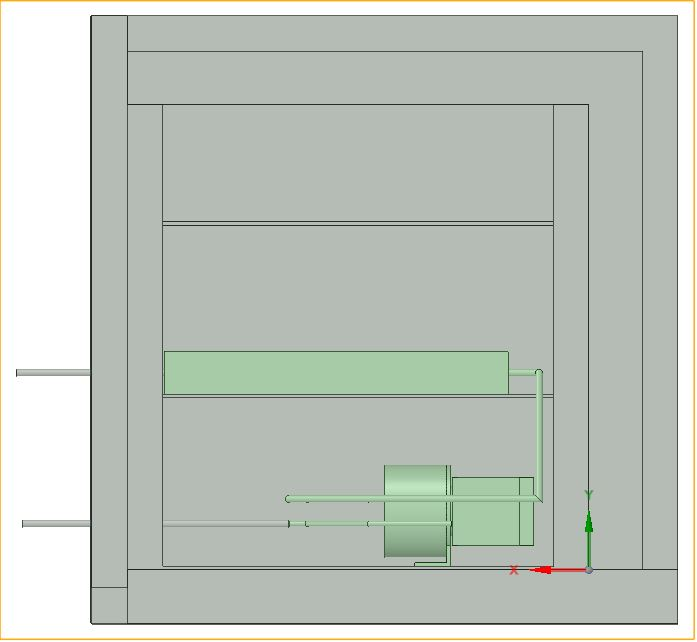
\includegraphics[width=0.5\linewidth]{appendix/img/Thermal/CAD-ansys.JPG}
    \end{align*}
    \caption{The CAD Model Used for ANSYS Simulations}
    \label{fig:Ansys-CAD-model}
\end{figure}

In ANSYS, FEA simulations were done using both Steady-State Thermal and Transient Thermal analysis.
Because of the limitations in ANSYS student license, a simplified model was used, which can be seen in Figure \ref{fig:Ansys-Brain-model}. It was focused on the corner region of the experiment housing the Brain and had three walls to the sampling bags and assumed the air was uniformly heated on the inside. The uniform inside air could be taken from the data from the test flight in Figure (\ref{fig:thermal-testflight-AAC}). These simulations were done to find what temperature the pump and manifolds would reach, as they were the most critical components in the experiment.

A transient thermal analysis was also performed by simulating a test flight with data from BEXUS 25 using results from MATLAB. It was performed so the thickness of the wall could be verified to see if it was good enough and whether adding heaters was required. Through the addition of, correct placement, adequate assigned power, and activation time for the heaters, it was possible to enable the pump and the manifold to operate in their required temperature ranges.

\subsection{ANSYS Result}
\subsubsection{Including Air With Same Density as Sea Level in the Brain}
\begin{figure}[H]
    \begin{align*}
        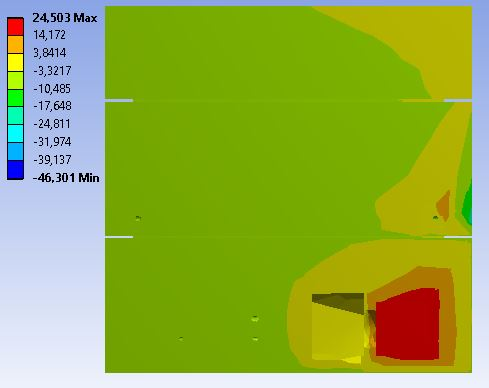
\includegraphics[width=0.5\linewidth]{appendix/img/Thermal/Air-inside-AAC-sampling-ascent.JPG}
    \end{align*}
    \caption{Cross Section of the Air in the Brain at the Time to Sample During Ascent.}
    \label{fig:Ansys-Brain-model} %Ivan was here
\end{figure}

\begin{figure}[H]
    \centering
    \subfloat{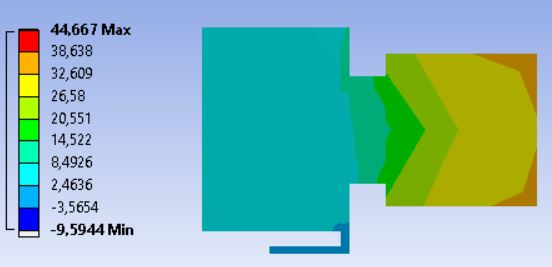
\includegraphics[width=0.49\linewidth]{appendix/img/Thermal/Pump-sampling-ascent.JPG}}
    \hifll
    \subfloat{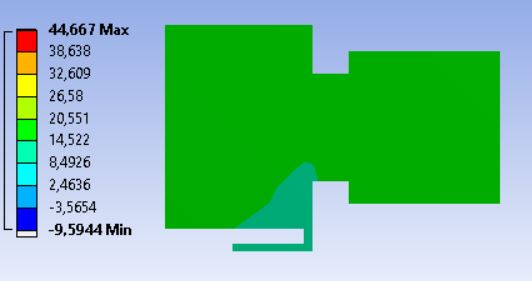
\includegraphics[width=0.48\linewidth]{appendix/img/Thermal/Pump-sampling-descent.JPG}}
    \caption{The Pump at the Time to Sample During Ascent (left) and Descent (right).}
    \label{fig:Pump-Valve-ascent-sample}
\end{figure}

\begin{figure}[H]
    \centering
    
    \subfloat{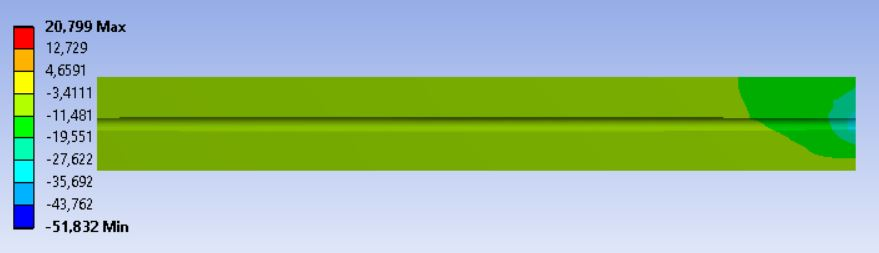
\includegraphics[width=0.48\linewidth]{appendix/img/Thermal/Valve-manifold-sampling-ascent.JPG}}
    \hifll
    \subfloat{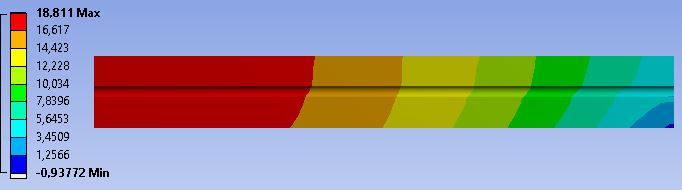
\includegraphics[width=0.50\linewidth]{appendix/img/Thermal/Valve-manifold-sampling-descent.JPG}}
    \caption{The manifold at the Time to Sample During Ascent (left) and Descent (right).}
    \label{fig:Pump-Valve-ascent-sample-descent}
\end{figure}

\begin{figure}[H]
    \centering
    \subfloat{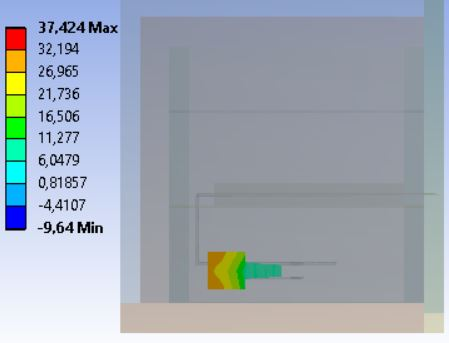
\includegraphics[width=0.43\linewidth]{appendix/img/Thermal/Critical-lowest-pump.JPG}}
    \hifll
    \subfloat{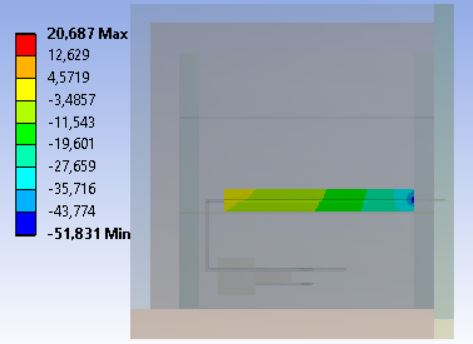
\includegraphics[width=0.45\linewidth]{appendix/img/Thermal/Critical-lowest-valve.JPG}}
    \caption{Pump and Manifold at the Coldest Part of Ascent.}
    \label{fig:Pump-Valve-ascent-critical-lowest}
\end{figure}

\begin{figure}[H]
    \begin{align*}
        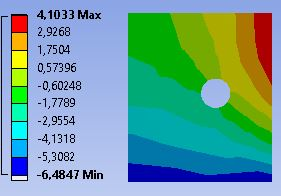
\includegraphics[width=0.5\linewidth]{appendix/img/Thermal/flushing-valve-ascent.JPG}
    \end{align*}
    \caption{Flushing Valve a Little Before Sampling Shall Start.}
    \label{fig:flushing-valve}
\end{figure}

\subsubsection{No Air in the Brain}

\begin{figure}[H]
    \centering
    \subfloat{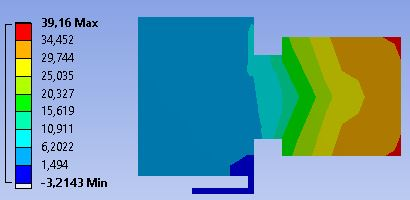
\includegraphics[width=0.49\linewidth]{appendix/img/Thermal/Pump-sampling-ascent-no-air.JPG}}
    \hifll
    \subfloat{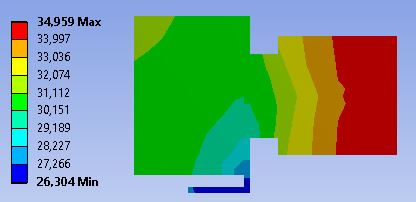
\includegraphics[width=0.49\linewidth]{appendix/img/Thermal/Pump-sampling-descent-no-air.JPG}}
    \caption{The Pump at the Time to Sample During Ascent (left) and Descent (right).}
    \label{fig:pump-no-air-in-brain}
\end{figure}

\begin{figure}[H]
    \centering
    \subfloat{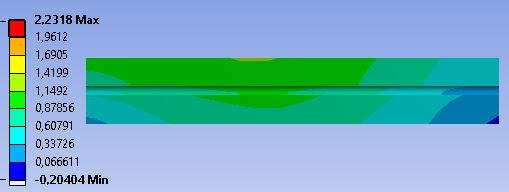
\includegraphics[width=0.44\linewidth]{appendix/img/Thermal/manifold-sampling-ascent-no-air.JPG}}
    \hifll
    \subfloat{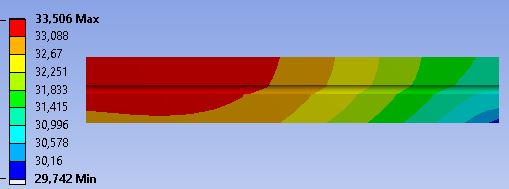
\includegraphics[width=0.442\linewidth]{appendix/img/Thermal/manifold-sampling-descent-no-air.JPG}}
    \caption{The manifold at the Time to Sample During Ascent (left) and Descent (right).}
    \label{fig:structure-no-air}
\end{figure}

\begin{figure}[H]
    \centering
    \subfloat{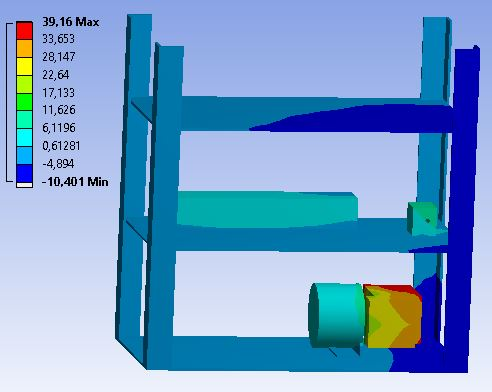
\includegraphics[width=0.44\linewidth]{appendix/img/Thermal/no-air-sampling-ascent.JPG}}
    \hifll
    \subfloat{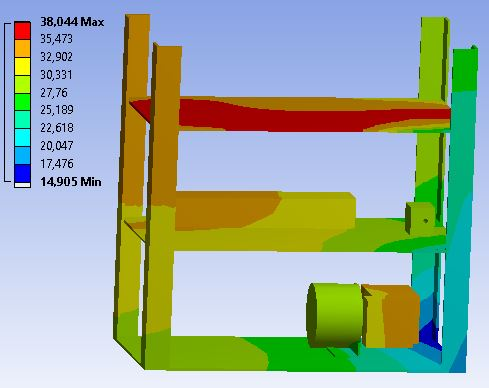
\includegraphics[width=0.442\linewidth]{appendix/img/Thermal/no-air-sampling-descent.JPG}}
    \caption{The Structure of the Brain at the Time to Sample During Ascent (left) and Descent (right).}
    \label{fig:structure-no-air2}
\end{figure}

\begin{figure}[H]
    \begin{align*}
        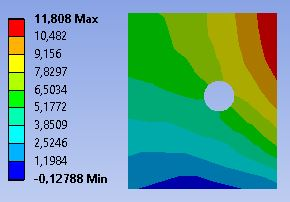
\includegraphics[width=0.5\linewidth]{appendix/img/Thermal/flushing-valve-no-air-ascent.JPG}
    \end{align*}
    \caption{Flushing Valve a Little Before Sampling Shall Start.}
    \label{fig:flushing-valve}
\end{figure}

\subsection{Result}
The main objective from first performing the MATLAB calculations and then the ANSYS simulations was to find the wall thickness of Styrofoam between the Brain and the inside of the AAC box and make updated iterations of the result. The next objective was to iterate the design by adding heaters to find the required amount and find approximately how long they need to run. By running a transient thermal analysis for the test flight it was possible to simulate heaters that will be on and off to determine how strong they need to be.

The results from the ANSYS simulations assumed a worst case scenario. It was to be expected that the results were not fully accurate, and instead were slightly warmer in reality. The worst case was with air inside the experiment at normal density. In reality when it was time to sample (at 17km), the air density would be less then 15\% of the air density at sea level \cite{EngToolair}. This meant that there would be less heat loss from components to the air inside the brain than predicted. Figures \ref{fig:Pump-Valve-ascent-sample} and \ref{fig:Pump-Valve-ascent-sample-descent} show that the temperature of the pump was above $5\degree{C}$ and the manifold was above $-10\degree{C}$. It was only during a portion of the Ascent Phase, just prior to the start of sampling that the heater would need to be on in order for the pump to be above $5\degree{C}$, and it would only need to be on during this Phase. By having a heater on the flushing valve and the manifold it was possible to get all the valves to the operating temperature. The flushing tube that led out to the open air outside would cool down the flushing valve, so a heater there to compensate for the heat loss would be required. It would then be time to flush right before sample can be seen in Figure \ref{fig:flushing-valve}. The manifold would still need a heater because it will be affected by the cold outer air and help heat up all the components.

The insulation for the AAC used is specified in Table \ref{tab:Wall-thickness-AAC-CAC}. For the three inner walls between the Brain and the bags there was a $0.03 m$ long wall of Styrofoam. Two $5\,W$ heaters for the pump (one on top and one on bottom side), a 5 W heater for the flushing valve and one for the manifold were used. The thermal simulations predicted that they would be within the operating limits with a satisfactory margin. For the heater controller, it would be set such that if the pump fell below $15\degree{C}$, it would turn on. As for the flushing valve, the heater would be set to turn on if the flushing valve and manifold fell below $-5 \degree{C}$.

%The insulation elements will be attached to the rails and to each other through the use of glue as an adhesive. Due to its strength, glue can provide sufficiently strong bonds over small areas of contact between materials. This means only a handful of additional heat bridges to be factored and none of them particularly conductive. For remaining portions near the edges of each wall of insulation, the materials may be connected together with tape owing to its adhesive strength being similar to that of the glue. The tape would prevent convection (at the cost of slightly increased conduction at the points/edges of contact) at lower altitudes from occurring due to air flowing in between the otherwise exposed gaps between the Styrofoam, the aluminum sheets, and the rails. In the event that tape would not be a suitable candidate, the Styrofoam may be milled to match the groove profile of the supporting rails so that it may be fitted in between them directly - leaving the whole structure secure while only using glue for connecting the Styrofoam to the aluminum sheeting.

%The Styrofoam will be attached to the structure with thread. By attaching a thread to the 90 degree bracket reinforcements (seen in Figure \ref{fig:corner_bracket}) and then tie them together at the middle. Together with the aluminum sheet screwed into the structure it will make a slot to keep the Styrofoam in place so it can not move around. By having the thread tied in the middle it is possible tighten it up.

%Thread will be used to attache the styrofoam to the structure. It will loop around the 90 degree bracket reinforcements (seen in Figure \ref{fig:corner_bracket}) and its ends will be tied together in between them. Together with the aluminum sheet screwed into the structure, the thread will make a slot to keep the Styrofoam in place, keeping the styrofoam block held in place. By having the thread knot(s) in the middle it will be possible for the thread to be tightened to any degree necessary to prevent insulation instability.
